\chapter{Resultados Experimentais }
\label{cap:resultados}

\section{Resultados}


\subsection{RC3, RC7 e RC28}

Assim como proposto em \cite{greciaLin}, iremos usar dados supostos disponíveis diariamente no chão de fábrica. Portanto, para um lote recém expedido,
não podemos usar os índices RC3 e RC7 para auxiliar na predição de RC28. Dessa maneira, iremos usar os últimos índices RC3 e RC7 disponível para o lote expedido no dia $t$,
i.e. o índice RC3 do dia $t-3$ e RC7 do dia $t-7$, que acabaram de ser medidos. 

\subsection{Divisão dos dados entre treino e validação}

\begin{figure}[H]
  \centering
  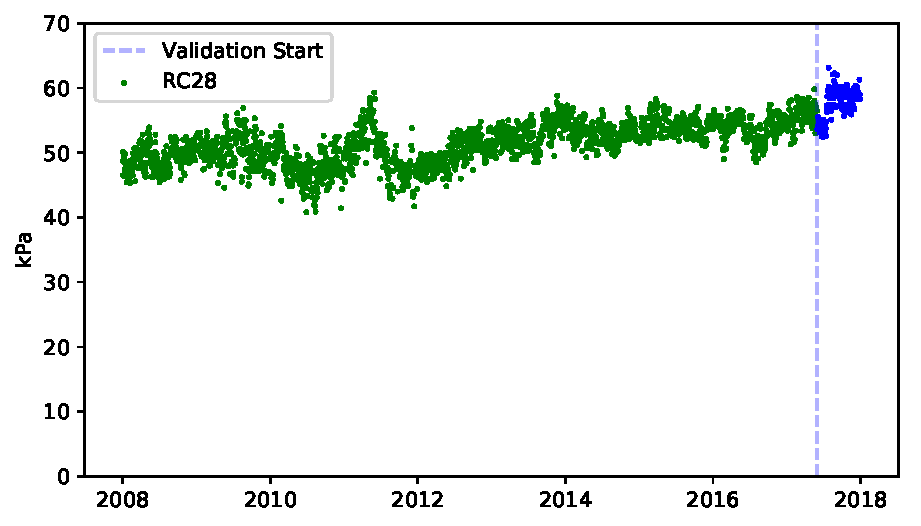
\includegraphics[width=0.9\columnwidth]{train_dev.pdf}
  \caption{Divisão do dataset para a saída RC28, os pontos verdes foram usados para
    treino e os pontos azuis usados para validação.}
  \label{fig:divrc28}
\end{figure}

\subsection{Abordagem Não-Temporal}

Modelos de Machine Learning não-temporais foram usados para treinar e validar os dados, para esses modelos usamos a biblioteca Sklearn.
As avaliações de RMSE de todo o conjunto de validação estão apresentados por modelos na Imagem~\ref{fig:linmodels}  

\begin{figure}[H]
  \centering
  \label{fig:linmodels}
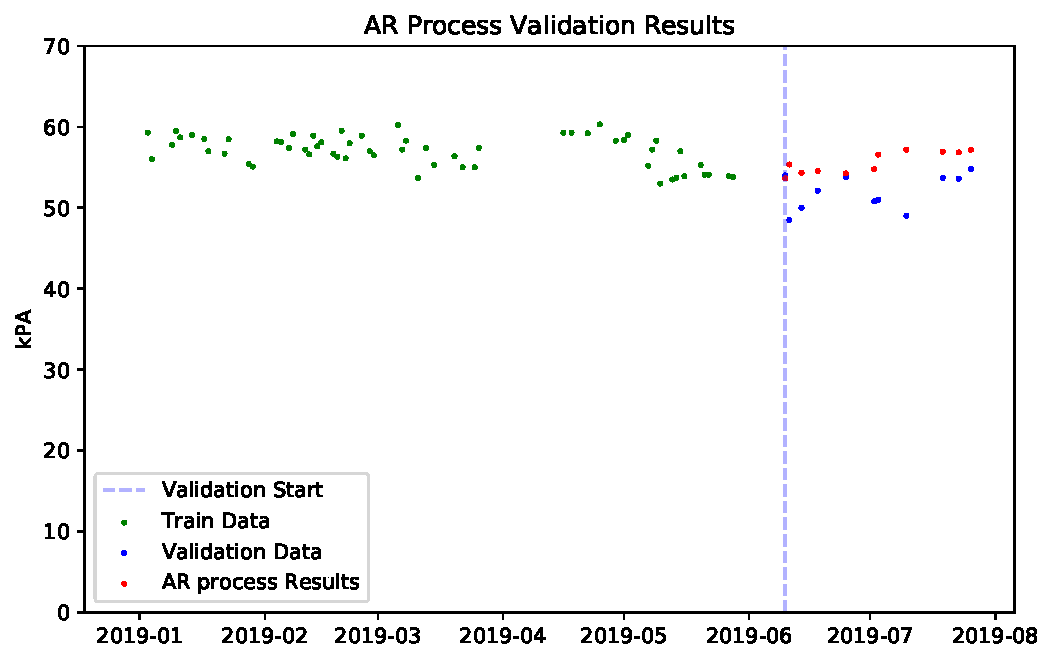
\includegraphics[width=0.9\columnwidth]{linear_exp.pdf}
\caption{Predições nos dados de validação nos experimentos com modelos não-temporais. }
\end{figure}

\subsection{Regressão Linear Dinâmica com Filtragem Exponencial}

Para efeito de comparação de resultados, iremos aplicar o método proposto em
\citep{grecialin}. Primeiramente apresentamos a variação do erro de treino em
função do parâmetro $t_d$ i.e. o tamanho do conjunto de treino para cada
regressão.

\begin{figure}[H]
  \centering
  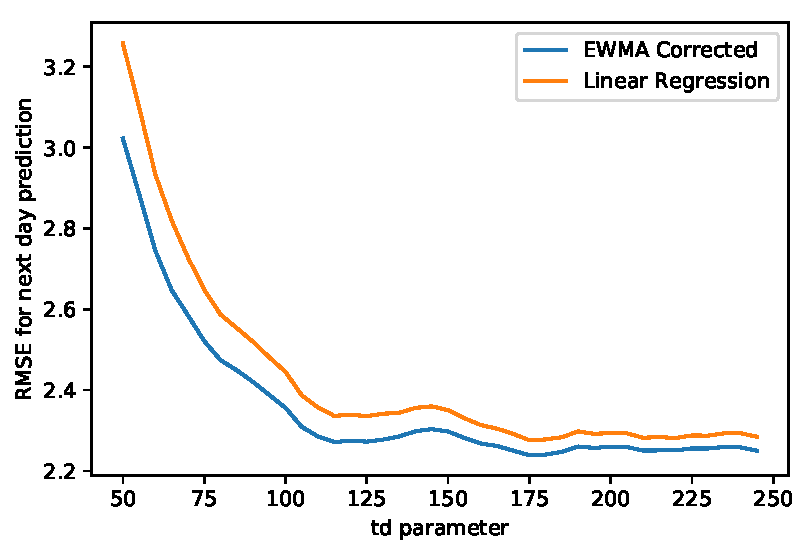
\includegraphics[width=0.9\columnwidth]{tdparameter.pdf}
  \caption{Erro de treino em função do parâmetro $t_d$}
  \label{fig:tdparam}
\end{figure}

Os resultados do modelo em todo o período de validação, bem como o erro são
reportados a seguir:

\begin{figure}[H]
  \centering
  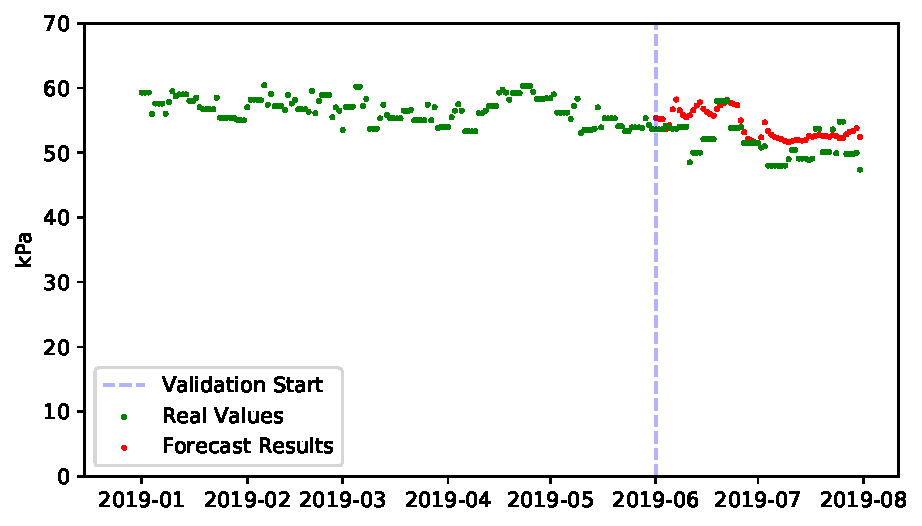
\includegraphics[width=0.9\columnwidth]{forecast_lin_reg_win.pdf}
  \caption{Predições no conjunto de validação do modelo de regressão linear dinâmico}
  \label{fig:tdparam}
\end{figure}

\subsection{Modelos Bayesianos para Séries Temporais}


Todos os modelos foram implementados usando a biblioteca Pytorch \cite{pytorch}, para os Processos Gaussianos usamos a biblioteca GPyTorch \cite{gpytorch}. As tuplas de treino são da forma $(RC28_{t},\{\})$. 

Para os modelos DeepAR e Encoder-Decoder-Forecaster, as predições começam após uma janela inteira de dias ser codificada pelas redes Encoder. Apenas então os modelos terão informação para gerar predições. O Modelo Deep Factors não necessita de uma janela pois sua arquitetura permite e emissão de predições imediatamente após o primeiro timestep ser recebido, e o Processo Gaussiano gera incertezas para todo o dataset de validação ao mesmo tempo, visto que é uma operação matricial. \\

As Imagem \ref{fig:rmseday}, mostra o RMSE médio dos modelos por dia a medida que o horizonte de predição aumenta. A Tabela \ref{tab:rmse} mostra o mesmo resultado porém apenas para a predição de 24h, 3d e 7d. \\



\begin{figure}[H]
\label{fig:rmseday}
\centering
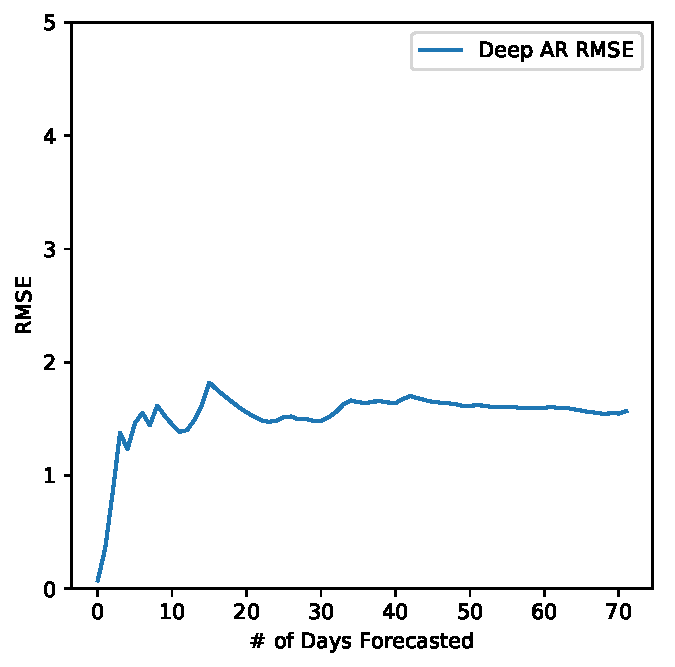
\includegraphics[width=.3\textwidth]{rmse_deep_ar.pdf} \hfill
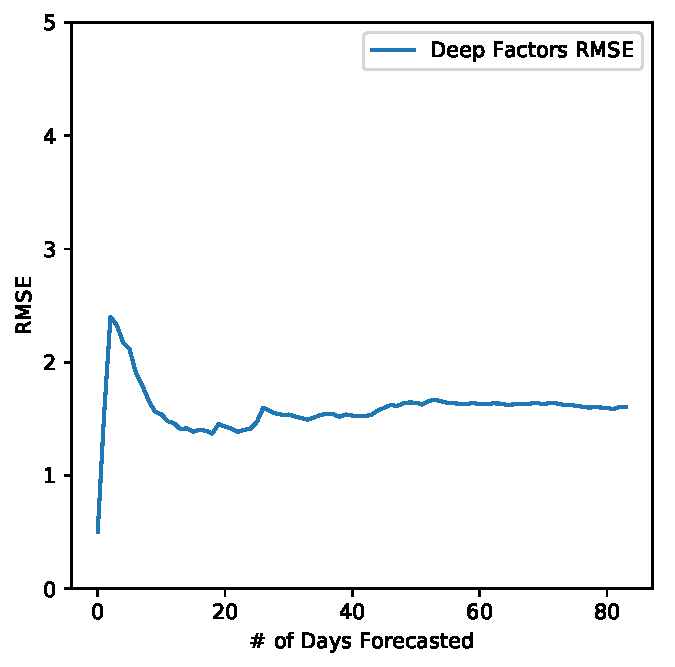
\includegraphics[width=.3\textwidth]{rmse_deep_factors.pdf} \hfill
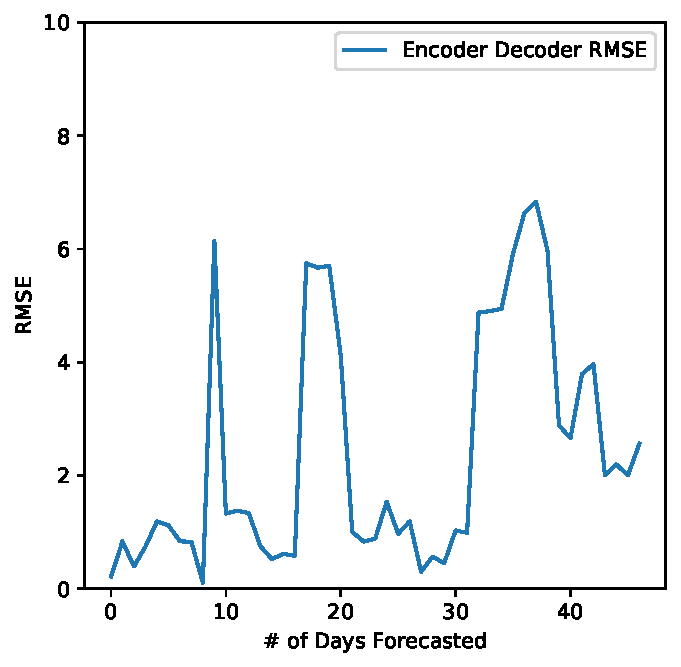
\includegraphics[width=.3\textwidth]{rmse_enc_dec.pdf} 
\caption{RMSE médio por dia para cada um dos modelos estudados} 
\end{figure}


\begin{center}
\begin{table}[htbp]
\caption{\label{tab:rmse}
RMSE values by forecast span}
\centering
\begin{tabular}{rr}
\hline
Deep Factors & RMSE\\
\hline
24h & 0.18\\
3d & 2.36\\
7d & 1.83\\
\hline
Deep AR & RMSE\\
\hline
24h & 0.07\\
3d & 1.37\\
7d & 1.44\\
\hline
Encoder Decoder & RMSE\\
\hline
24h & 0.22\\
3d & 0.36\\
7d & 1.04\\
\end{tabular}
\end{table}
\end{center}


Também estudamos a distribuição dos valores previstos, até 150 dias após a data onde começam os dados de validação, a Imagem \ref{fig:distr} permite comparar as distribuições previstas pelos 3 modelos:

\begin{figure}[H]
\label{fig:distr}
\centering
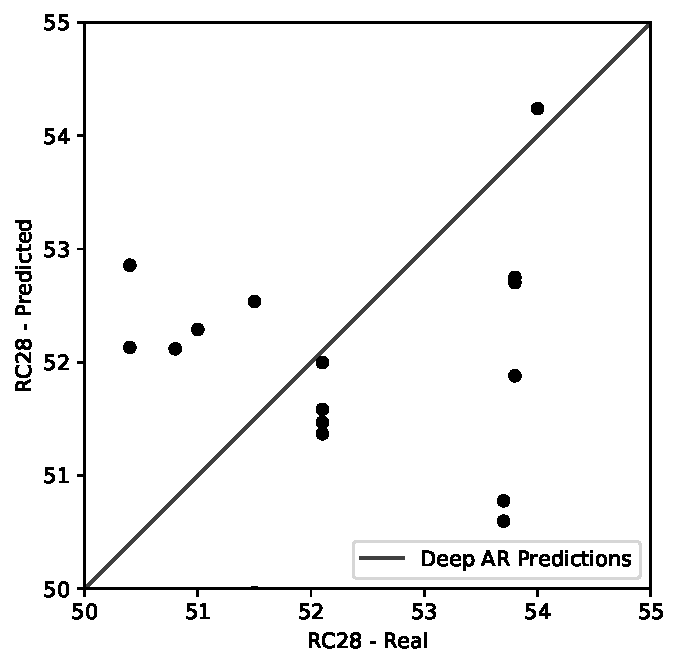
\includegraphics[width=.3\textwidth]{qq_deep_ar.pdf} \hfill
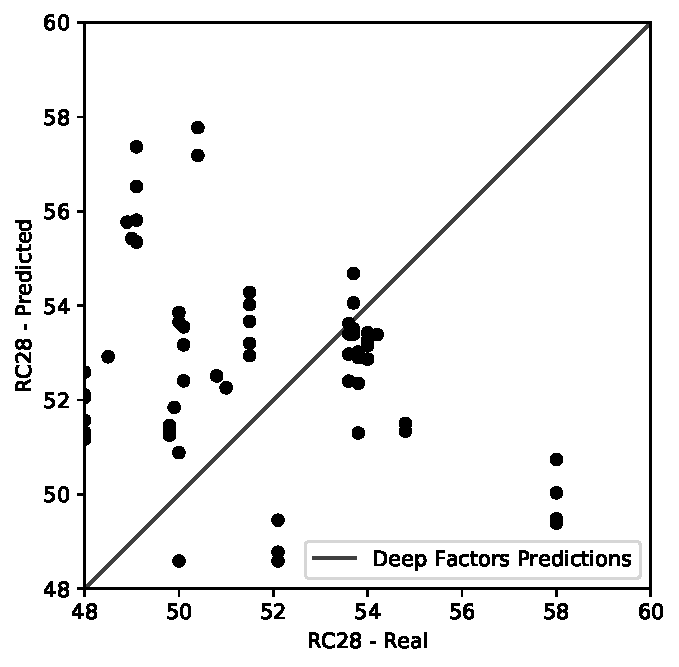
\includegraphics[width=.3\textwidth]{qq_deep_factors.pdf} \hfill
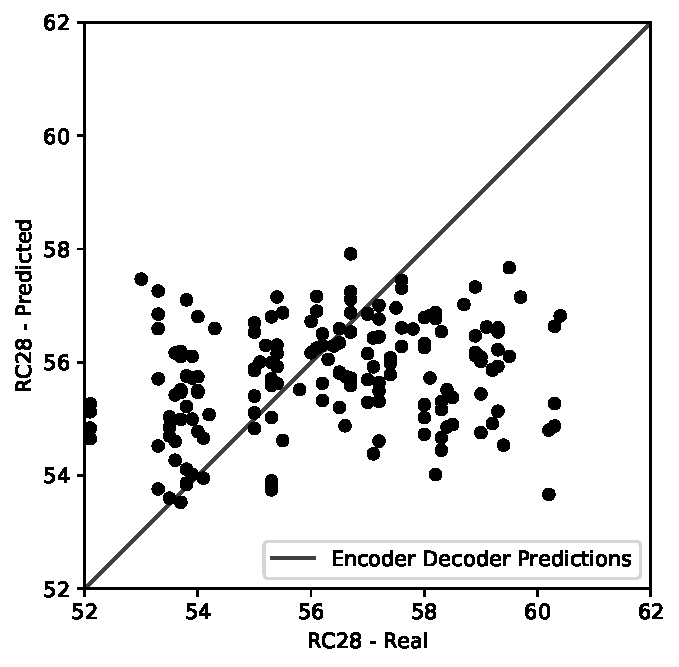
\includegraphics[width=.3\textwidth]{qq_enc_dec.pdf} 
\caption{Valores reais plotados contra os valores previstos para análise da distribuição aprendida por cada modelo} 
\end{figure}


Finalmente, os valores e incertezas previstos pelos modelos:


\begin{figure}[H]
  \label{fig:fordeepar}
  \centering
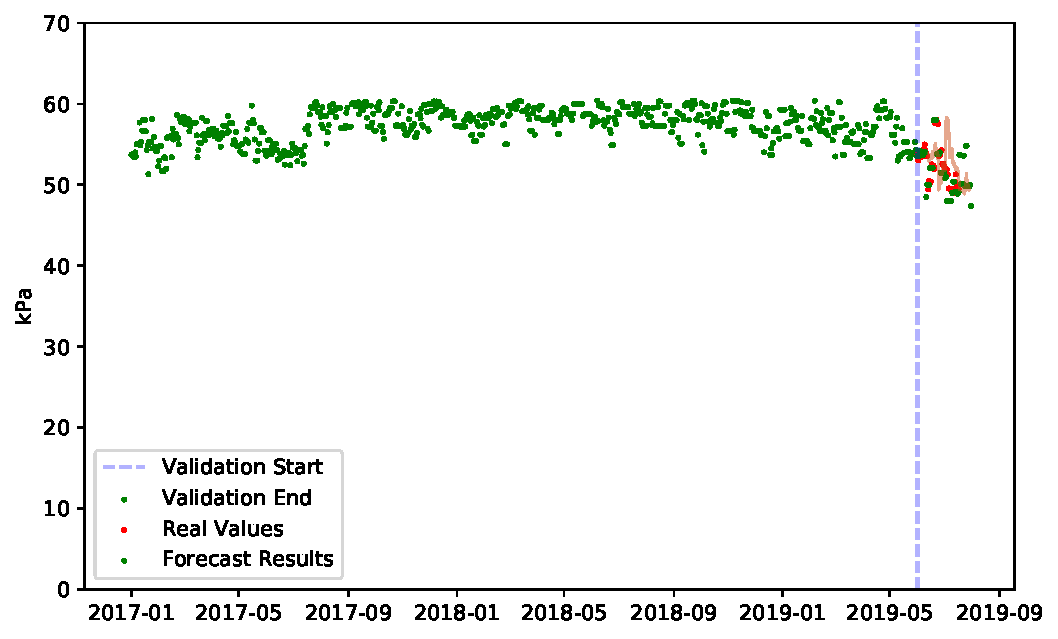
\includegraphics[height=.3\textwidth]{forecast_deep_ar.pdf} 
\caption{Predição para todos os dados de validação para o modelo Deep AR}
\end{figure}

\begin{figure}[H]
  \label{fig:fordeepfactors}
  \centering
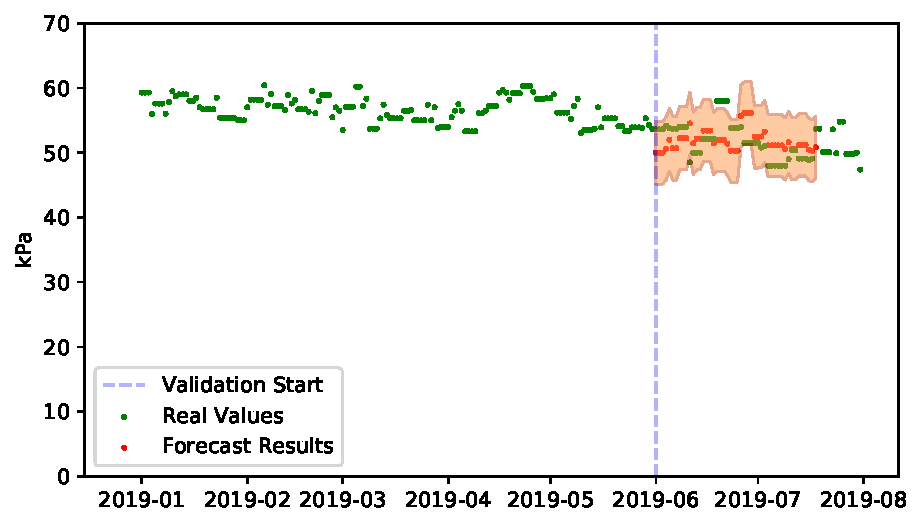
\includegraphics[height=.3\textwidth]{forecast_deep_factors.pdf} 
\caption{Predição para todos os dados de validação para o modelo Deep Factors}
\end{figure}

\begin{figure}[H]
  \label{fig:forencdec}
  \centering
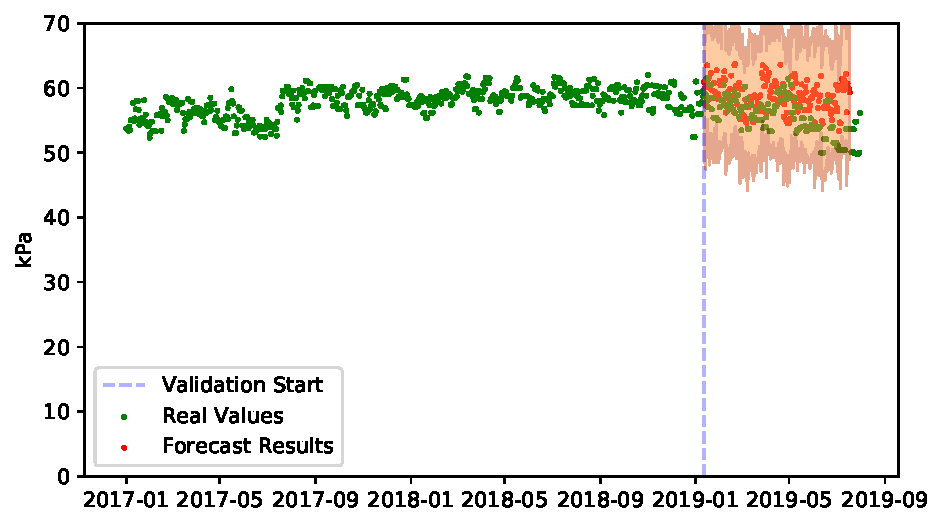
\includegraphics[height=.3\textwidth]{forecast_enc_dec.pdf} 
\caption{Predição para todos os dados de validação para o modelo Encoder Decoder Forecaster} 
\end{figure}


Para modelagem de séries temporais, é também comum estudarmos o resíduo das predições. A sua distribuição deve ser randômica para garantirmos que nosso modelo não está cometendo algum viés que seria
modelável com mudanças no aprendizado. \\


\begin{figure}[H]
\label{fig:distr}
\centering
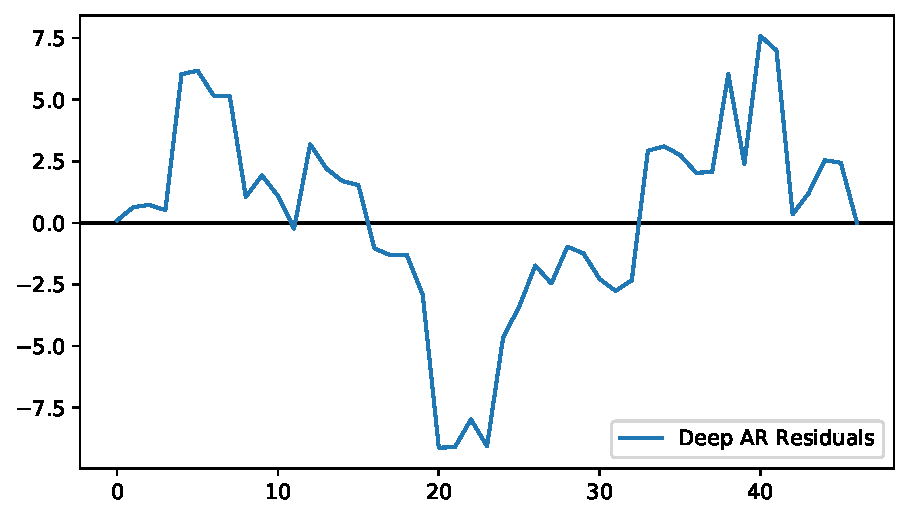
\includegraphics[width=.3\textwidth]{res_deep_ar.pdf} \hfill
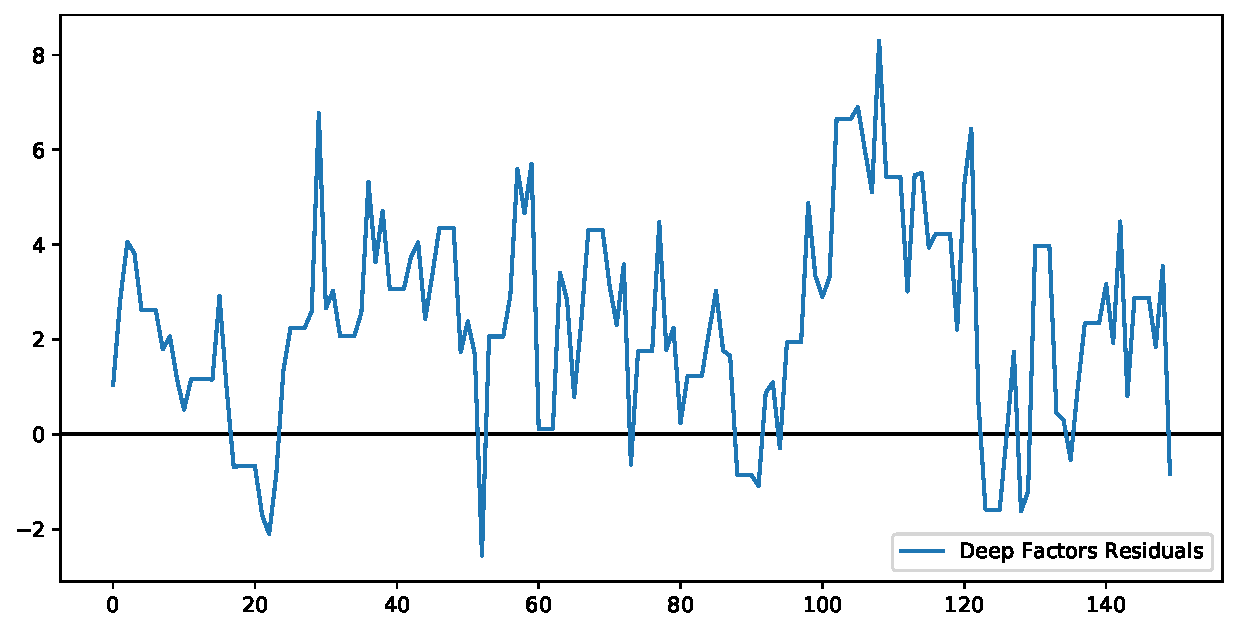
\includegraphics[width=.3\textwidth]{res_deep_factors.pdf} \hfill
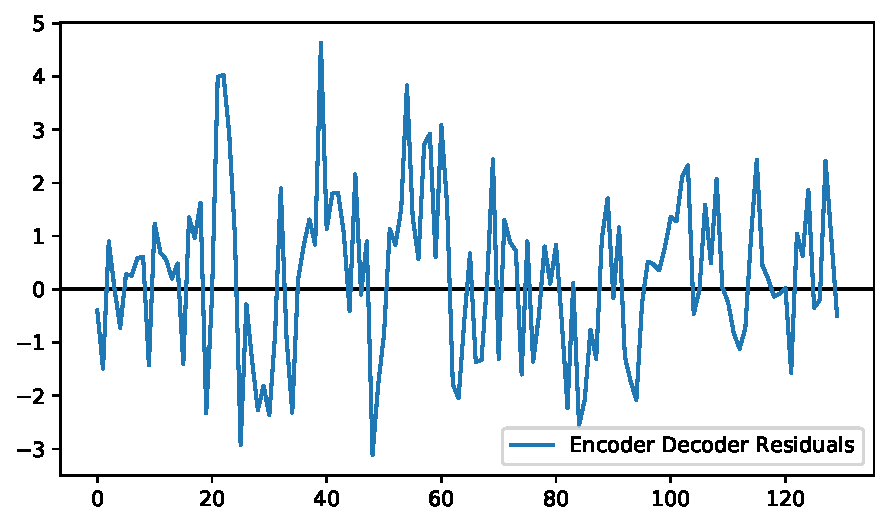
\includegraphics[width=.3\textwidth]{res_enc_dec.pdf} 
\caption{Distribuição dos Erros de cada modelo. Como esperado, todos os erros flutuam em torno da média 0. } 
\end{figure}



% Local Variables:
% TeX-master: "../quali"
% End:
